
    In conclusion, this thesis demonstrates the feasibility and potential of using transformer-based models for texture generation in video game development and use. The Column Image Transformer (CIT) and Spiral Image Transformer (SIT) represent initial approaches and potential ways in which traditional Transformer architectures can be extended beyond text to graphical content generation. Each model offers unique benefits and poses different challenges. Both models require further development to become fully user-friendly and capable of generating assets efficiently.

\subsection{Evaluation of the Models}

    As a general conclusion, the data suggest that it is possible to quickly generate new assets through this approach. Especially the CIT model can generate new assets in a short amount of time because it does not process the whole image at once and is highly parallelizable. However, this is also a significant disadvantage because it is unable to envision the whole context. In contrast, the Spiral Model, which can see the entire image at once, is unable to generate new assets quickly due to the fact that all pixels need to be generated after another. The best approach might be to find a middle ground between the two models. For example, using a wider width than in the CIT model or feeding additional information to the model, such as the x position of the pixel to be generated.

    Another addition to the model could be the use of text input as additional information. This would be a good approach to generate more specific assets and it would be easier to start from no or a smaller amount of seed pixels, similar to DALL-E or Midjourney.

    \subsubsection{Quality and image generation}
    This section focuses on the generation of images. Two cases are presented below. The first case involves the generation of high-quality images, where the CIT model is used. In this example, the model continues to generate the image from a 511x511 image source.
    
    The second case addresses the generation of pixel art or low-resolution images, where both the CIT and SIT models are used. These textures could be used in games like Minecraft, Terraria, or Stardew Valley, where the style relies on a low resolution and pixel art style.

    \newpage
    \begin{itemize}
        \item \textbf{High-Quality Image Generation:}
    
            The following image displays four randomly selected images from the dataset. The CIT model processes the upper part of the image and then generates the lower part, which is marked with a purple background.
    
            \begin{figure}[H]
                \centering
                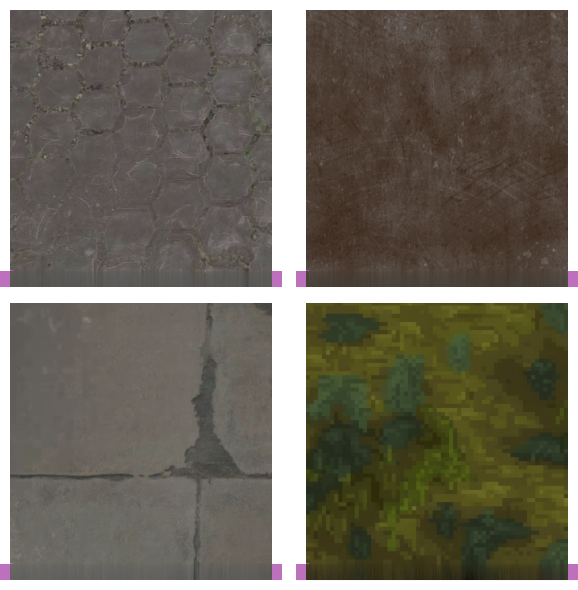
\includegraphics[width=0.7\textwidth]{imgs/GenExample1.png}
                \caption{Four images with lower parts generated by the CIT [model 4]}
                \label{fig:GenExample1}
            \end{figure}
    
            As shown in the image above, the model requires a significant amount of seed pixels to generate a high-quality image. A problem arises when only a few seed pixels are used. Often, the model generates a solid-filled image or slowly changes the context to a different texture or presumably random noise. This issue could be addressed by using a wider context window in the x-direction or by feeding additional information to the model.
    
        \item \textbf{Pixel Art / Low-Resolution Image Generation:}
        
            The following two images illustrate the generation of pixel art or low-resolution images 32x32 pixels. The first image displays a kelp or mossy type texture generated by the CIT model and the second image shows a dark brick-like texture generated by the SIT model.
    
            \begin{figure}[H]
                \centering
                % First image
                \begin{minipage}{0.30\textwidth}
                    \centering
                    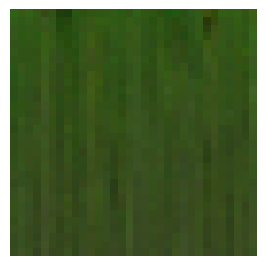
\includegraphics[width=\textwidth]{imgs/GenExample2.png} 
                    \subcaption{Kelp texture CIT [model 4]}
                    \label{fig:GenExample2}
                \end{minipage}
                \hspace{0.05\textwidth} % Adjust spacing between images
                \begin{minipage}{0.30\textwidth}
                    \centering
                    
\includegraphics[width=\textwidth]{imgs/GenExample3.png} 
                    \subcaption{Dark brick texture SIT [model 6]}
                    \label{fig:GenExample3}
                \end{minipage}
                \caption{Two low-resolution images generated by the CIT and SIT models}
                \label{fig:GenExample2_3}
            \end{figure}
            
            Both images are generated from a small amount of seed data. The image in \autoref{fig:GenExample2_3} (1) is seeded with a 6x32 pixel image quickly created in Microsoft Paint with a pattern roughly matching the output colors but lacking structure and smooth transitions.
    
            The image in \autoref{fig:GenExample2_3} (2) was seeded with an inner 5x5 pixel image, created similarly to the process above.
    \end{itemize}
    
    

\subsubsection{Performance}

    A key question that arises is whether it is feasible to generate assets for video games using the developed models. This question can be divided into two distinct parts. The first considers the pre-generation of assets during the development cycle, while the second evaluates whether the models are efficient enough to generate assets in real-time on a local machine.

    The following table provides a detailed overview of the performance metrics for the CIT and SIT models, tested on both GPU and CPU. It is noteworthy that the Tokens column refers to the number of tokens used for generating the image. The CIT model utilizes a batch size of 32 and a context length of 32 tokens, while the SIT model uses a batch size of 1 and a context length of 1024 tokens. Both models generate a resulting image of 32x32 pixels. Each model was tested on a local workstation equipped with an NVIDIA GeForce RTX 3090 GPU and an AMD Ryzen 9 7900X CPU.

    \begin{table}[H]
        \centering
        \small
        \begin{tabular}{|l|c|c|c|c|}
        \hline
        \textbf{Model} & \textbf{Platform} & \textbf{Total Time (sec)} & \textbf{Avg Time per Token (sec)} & \textbf{Tokens} \\ \hline
        \multirow{2}{*}{CIT [1] 128} & GPU & 0.511 & 0.000499 & \multirow{2}{*}{32x32} \\ \cline{2-4}
                                           & CPU  & 0.494 & 0.000483 &  \\ \hline
        \multirow{2}{*}{CIT [3] 256} & GPU & 0.725 & 0.000708 & \multirow{2}{*}{32x32} \\ \cline{2-4}
                                           & CPU  & 2.851 & 0.002784 &  \\ \hline
        \multirow{2}{*}{CIT [4] 512} & GPU & 0.899 & 0.000877 & \multirow{2}{*}{32x32} \\ \cline{2-4}
                                           & CPU  & 4.489 & 0.004384 &  \\ \hline
        \multirow{2}{*}{SIT [5] Small} & GPU & 9.388 & 0.009168 & \multirow{2}{*}{1x1024} \\ \cline{2-4}
                                             & CPU  & 30.709 & 0.029989 &  \\ \hline
        \multirow{2}{*}{SIT [6] Big} & GPU & 15.773 & 0.015403 & \multirow{2}{*}{1x1024} \\ \cline{2-4}
                                           & CPU  & 114.394 & 0.111713 &  \\ \hline
        \end{tabular}
        \caption{Performance metrics for CIT and SIT models [local workstation]}
        \label{tab:performance_metrics}
    \end{table}
        
    The results indicate that the SIT model is significantly slower than the CIT model, especially when running on the CPU. This is due to the fact generating a bigger image in the batch dimensions is far more efficient than in the token dimension. For a detailed visualization of the performance scaling across these dimensions, refer to \autoref{fig:performanceTest} for batch dimension scaling and \autoref{fig:performanceTest2} for context dimension scaling on the CIT [model 4].

    It can be observed that both methods could be somewhat viable in a development environment where developers generate assets during the prototyping or development cycle. As shown in \autoref{fig:performanceTest}, the expected optimal runtime per pixel for the CIT model is 2.51 milliseconds. This would result in an approximate runtime of roughly 11 minutes for a 512x512 image on an RTX 3090 GPU.
    
    However, this could pose a challenge when considering running these models on an average gaming-capable machine. Due to the large amount of data and the size of the models, substantial video memory is required. Only 27.17\% of users have more than 8 GB of VRAM, and 49.37\% have at least an NVIDIA GeForce RTX 2060, according to the Steam Hardware Survey of March 2024 \autocite{Valve2024}. This could be problematic for the SIT model, which demands considerable memory to operate effectively. The CIT model could run on most machines, but the size/context length of the generated images would be compromised, and any enhancements to the model could further increase system requirements. Thus, a cloud-based solution might be a better approach for this case, when the created games should be capable of generating assets on the fly.
    

\subsection{Further research}

    The following section outlines potential areas for further research that could lead to significant improvements in model performance and usability and extend their applicability in real-world applications.

    \subsubsection{Discriminator}
    To achieve better results, a discriminator could be used to enhance the output of the model. In this context, a discriminator is a type of neural network trained to distinguish between real data and artificially generated data. The goal of the discriminator is to accurately classify data as either real from the actual dataset or fake, created by another neural network called the generator, in this case, the CIT or SIT Model. The discriminator's performance helps improve the generator, leading to more realistic synthetic data over time. In a perfect scenario, the discriminator cannot distinguish between the generated content and the original content, and the loss will balance out at 0.5 for the discriminator. This is the point where the generator is creating content indistinguishable from the original content.

    Some tests have been conducted with a discriminator and the CIT model, where the CIT model was pretrained to learn basic generation and then further trained with the discriminator. The tests indicated that the performance of the CIT model could be slightly improved and needs further investigation.

    \subsubsection{Incorporating Text Input}

    Integrating text input into an image generation model like the CIT or SIT could significantly enhance its functionality and usability by allowing the model to generate images based on descriptive text prompts. Unfortunately, due to time constraints, this feature was not implemented in this thesis, but it could be a valuable addition to the models. To implement this, all the data would need to be additionally labeled with text descriptions. Most of the images already contain basic descriptions in their names, such as "concrete floor" or "oak wood tiling," but further labeling and more data would be required. This would allow the model to generate images based on text input. The text input could be used to generate more specific assets or to create assets from scratch without any seed pixels. This would make the model more usable in the development process of video games.

    \subsubsection{LLM Scaling Laws}

    As often mentioned in this thesis, the lack of training data and potentially the small size of the models could be reasons for the models not performing perfectly. The scaling laws of LLMs \autocite{kaplan2020scaling} could potentially be applied to the CIT and SIT models to improve their performance. The scaling laws of LLMs suggest that the performance of a model can be improved by increasing the model's size and the amount of training data. This could be achieved by increasing the model's parameter count and the amount of training data. One way would be to increase the number of attention heads or the size of the feedforward network or by adding more transformer layers. 
    
    The amount of training data could also be increased by using more video game assets. In this thesis, 30 video games are used. Scaling up the training dataset and increasing the parameter count resulted in better outcomes, especially for the SIT model.
